% !TEX TS-program = LuaLaTeX
\documentclass[11pt,compress,xcolor=x11names,UTF8]{beamer}
\usetheme{Boadilla}
\usecolortheme{seahorse}
\useinnertheme[shadow]{rounded}  
\useoutertheme[subsection=false]{smoothbars}
\usecolortheme{spruce}
\usecolortheme[named=SpringGreen4]{structure}
\usefonttheme{structurebold}
\useinnertheme{circles}
\usecolortheme{rose}
\usepackage{pifont}
\usepackage{academicons}
\usepackage{fontawesome}
\usepackage{iitem}
%\usepackage{graphicx}
%\usepackage{tabular}
\setbeamertemplate{itemize item}{\ding{108}}
\setbeamertemplate{itemize subitem}{\ding{109}}
\setbeamertemplate{navigation symbols}{}
\setbeamercovered{transparent}  
\renewcommand\appendixname{附录}
\renewcommand\abstractname{摘要}
\graphicspath{{figure/}} % 图片路径
\usepackage{calligra} % Thank you
\usepackage{ctex} % 加入中文
%\setCJKsansfont{Noto Sans CJK SC}
\setsansfont{Lato} % Lato Roboto Fira Sans
\usepackage{makecell}
\newcommand{\tabincell}[2]{\begin{tabular}{@{}#1@{}}#2\end{tabular}}
\usepackage{url}					
\usepackage{natbib} % 参考文献
%\title[Spatial Generalized Linear Mixed Models]{Spatial Generalized Linear Mixed Models with Application to Prevalence Mapping}
\title{Container PMT Testing Data in ROOT format}
%\subtitle{奖助金申请答辩}
\author[Rong. Zhao]{Email:zhaor25@mail2.sysu.edu.cn \and  } % \\ 专业:统计学 \\ 方向:数据分析与统计计算
\institute[Sun Yat-Sen University]{School of Physics\and } % 理学院\\
\date[\today]{
\includegraphics[width=.5\textwidth]{logo}}

\begin{document}

\maketitle

%\begin{frame}{Outline}
%\tableofcontents
%\end{frame}

\section{Introduction}

%\subsection{研究意义}

\begin{frame}{motivation}
%\textsf{例} \textbf{例}  \textit{例} 
% \texttt{例}  % 调出仿宋字体了
	Due to complex of PMT testing procedure and upgrades of hardware and software, the raw data of PMT testing is not user-frinedly.
\vspace{.5cm}

	\alert{It is a good choice to produce a uniform structure to re-organize and store the raw data.}
%\begin{table}[]  
%\caption{PMT typical performance}  
%\resizebox{.8\textwidth}{!}{%
%\begin{tabular*}{.98\textwidth}{l|cccc}
%%\toprule  
%\hline  
%\hline  
%Performance & PDE &DCR & TTS& uniformity \\  
%\hline  
%HAMAMATSU &  lower\% & 20 kHz& 3ns& worse \\  
%NNVT  & higher\% & 40kHz & 7ns& better \\  
%\hline  
%\end{tabular*}  
%%}
%\end{table} 
%\begin{figure}
%\centering
%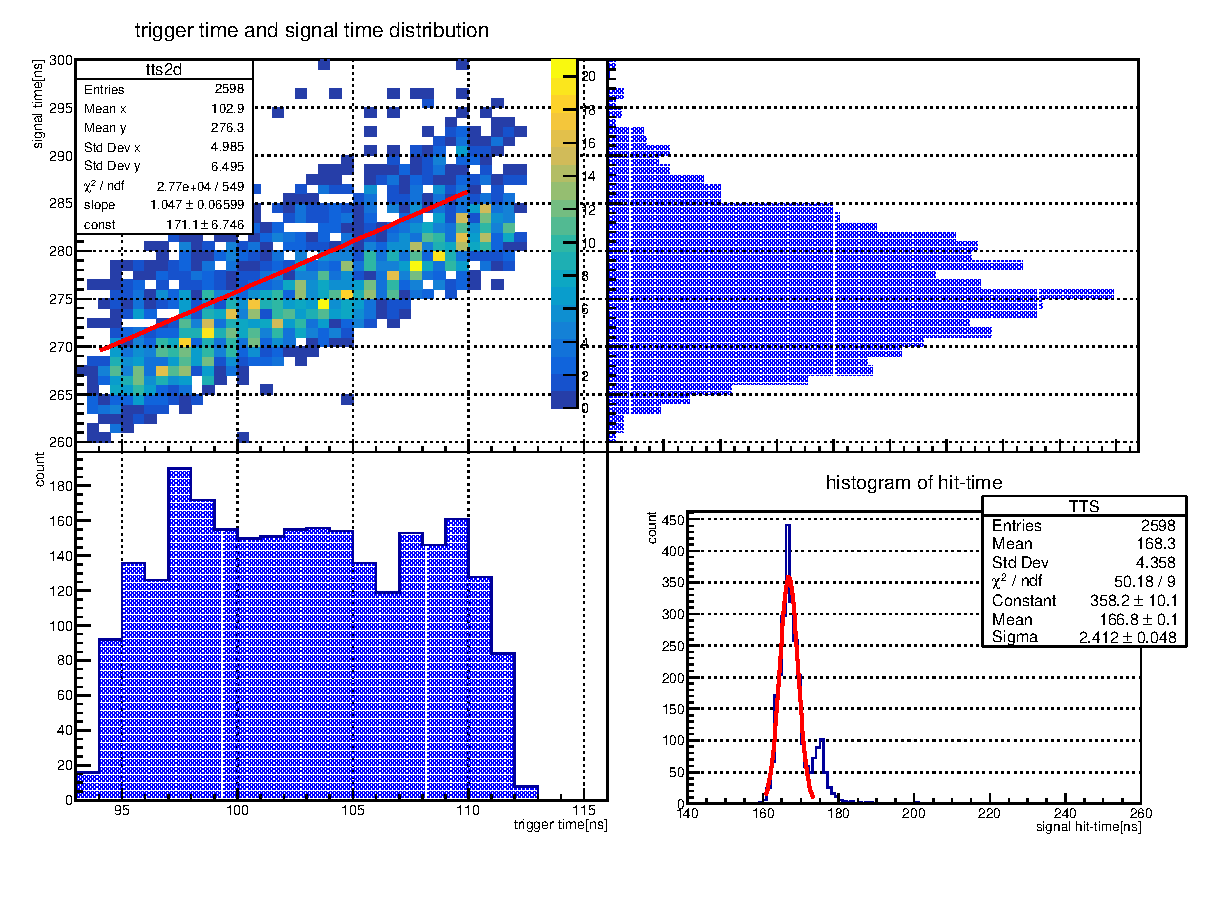
\includegraphics[width=0.78\textwidth]{typical_hittime} % 单图
%\end{figure}
\end{frame}
%%%%%%%%%%%%%%%%%%%%%%%%%%%%%%%%%%%%%%%%%%%
\begin{frame}{priliminary consideration}
	The minimum "object" of our container testing is \alert{drawer-test} rather than a spefcific PMT\footnote{since one PMT could be tested several times in different drawers due to failure of peformance test}.\\	
\vspace{.5cm}
the propertites:
	\begin{enumerate}
		\item  uniq \underline{testing number}
		\item validity of the data
	\end{enumerate}
\end{frame}
%%%%%%%%%%%%%%%%%%%%%%%%%%%%%%%%%%%%%%%%%%%
\begin{frame}{calibration of each drawer}
one root filesore the raw data, with branches: 0.1pewave,1pewave,ttswave,ttstrig,dcr,
\vspace{.5cm}
\hrule{\textwidth}
\vspace{.5cm}
a unique ID indicate the key info
\vspace{.5cm}
\end{frame}
\section{calibration of drawer}
%%%%%%%%%%%%%%%%%%%%%%%%%%%%%%%%%%%%%%%%%%%
\begin{frame}{how to calibrate}
The HAMAMATSU company has provided us with QE value of part of the PMTs, If we suppose the collection efficiency is same for all the HAMAMATSU PMTs we could use these QE values to calibrate drawers in the container.

\vspace{.5cm}
\hrule{\textwidth}
\vspace{.5cm}
In order to make sure the PDE-$\mu_{test}$ fitting results reasonable, only the PMT pass the test will be used for fitting.
\end{frame}
%%%%%%%%%%%%%%%%%%%%%%%%%%%%%%%%%%%%%%%%%%%
\begin{frame}{fitting example using 30 tubes}
\begin{figure}
\centering
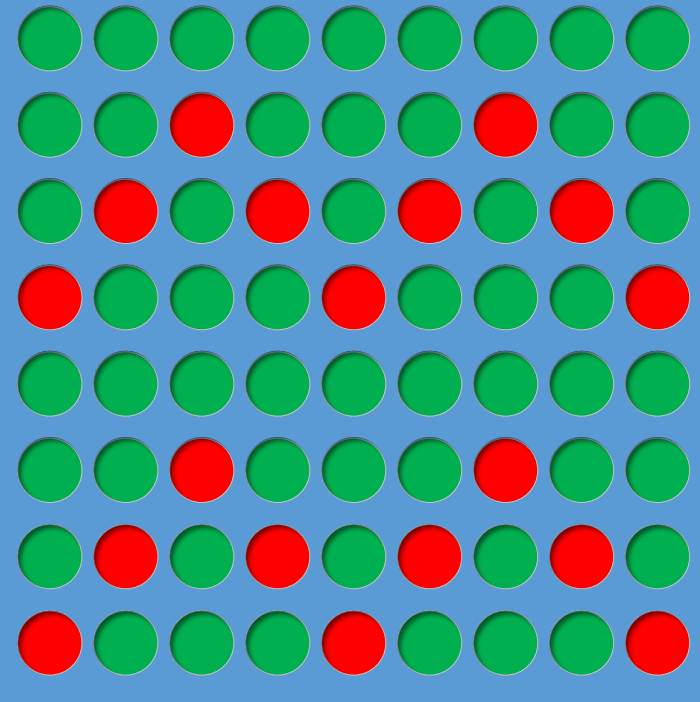
\includegraphics[width=0.58\textwidth]{pat5} % 单图
\end{figure}
results of more drawers can be found in the back-up part.
\end{frame}
%%%%%%%%%%%%%%%%%%%%%%%%%%%%%%%%%%%%%%%%%%%
%~~!!!!!!!!!!!!!!!!!!put two figures to illustrate!!!!!
\begin{frame}{drawer$_{factor}$ vs. PMT number drawer ###}
\begin{figure}
\centering
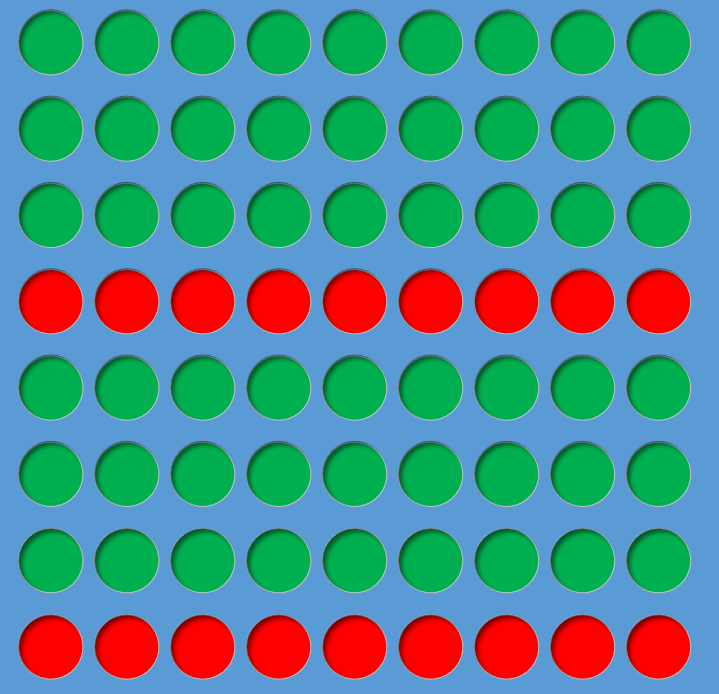
\includegraphics[width=0.58\textwidth]{pat3} % 单图
\end{figure}
more results can be found in the back-up part.
\end{frame}
%%%%%%%%%%%%%%%%%%%%%%%%%%%%%%%%%%%%%%%%%%%
\begin{frame}{discuss the results}
the relative error $e_{r}=\frac{f_{i}-f_{r}}{f_r}$ of one draw:
\begin{figure}
\centering
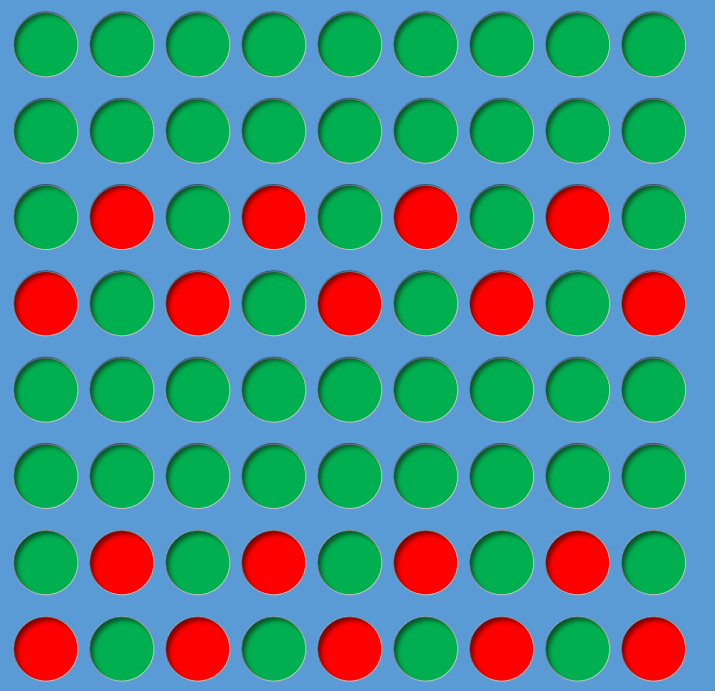
\includegraphics[width=0.58\textwidth]{pat4} % 单图
\end{figure}
define the first number that $|e_r|<1\%$ as $N_0$, we could get the $N_0$ value for each drawer.
\end{frame}
%%%%%%%%%%%%%%%%%%%%%%%%%%%%%%%%%%%%%%%%%%%
%%%%%%%%%%%%%%%%%%%%%%%%%%%%%%%%%%%%%%%%%%%
\begin{frame}{discuss the results}
\begin{figure}
\centering
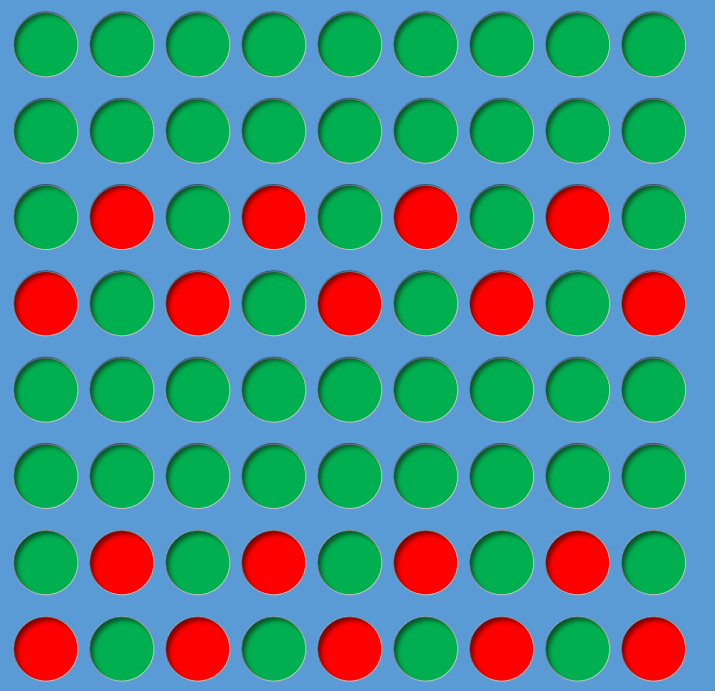
\includegraphics[width=0.58\textwidth]{pat4} % 单图
\end{figure}
This means we need to calibrate each drawer with  at least 30 PMTs to get a reliable drawer$_{factor}$.
\end{frame}

%%%%%%%%%%%%%%%%%%%%%%%%%%%%%%%%%%%%%%%%%%%%%%%%%%%%%%%%%%%%%%%%%%%%
\begin{frame}{ JUNO offline}
compare detector performance with the different PMT paterns, especially the time and energy resolution and reconstruction results.

\hrule{\textwidth}

how to:add method to the PMT class then each PMT can get its performance according to the layout pattern and its own ID. 
\end{frame}
%%%%%%%%%%%%%%%%%%%%%%%%%%%%%%%%%%%%%%%%%%%%%%%%%%%%%%%%%%%%%%%
\section{PMT orientation}
%%%%%%%%%%%%%%%%%%%%%%%%%%%%%%%%%%%%%%%%%%%%%%%%%%%%%%%%%%%%%%%%%%%%
\begin{frame}{HAMAMATSU PMTs}
the PDE uniformity of HAMAMATSU PMTs are not so good
\hrule{\textwidth}
we can artificially correct the PDE if these PMTs have fixed orientation and we can extract the light incident angle using reconstraction information.
\end{frame}
%%%%%%%%%%%%%%%%%%%%%%%%%%%%%%%%%%%%%%%%%%%%%%%%%%%%%%%%%%%%%%%


\begin{frame}
\centering {\zihao{0} \color{red} \calligra{Thank You}}

\end{frame}


%\begin{frame}[allowframebreaks]
%\frametitle{References}
%\scriptsize
%\bibliographystyle{authordate1}
%\bibliography{R-GLMM-pkgs}
%\end{frame}

\appendix

\section*{附录}

%\begin{frame}{Softwares and Tools}

%\includegraphics[width=.2\textwidth]{software/r}\qquad
%\includegraphics[width=.16\textwidth]{software/stan} \\ 
%\includegraphics[width=.45\textwidth]{software/bioconductor}
%\includegraphics[width=.45\textwidth]{software/PyMC3} 

%\end{frame}
%% OpenBUGS  WinBUGS  JAGS
% library(R2OpenBUGS) # 2017-2-20 version 3.2-3.2
% library(R2WinBUGS) # 2015-07-29 version 2.1-21
% library(rjags) # 2016-02-19 version 4-6
% library(BRugs) # OpenBUGS 2017-06-26  version 0.9-0
% library(glmmBUGS) # Generalised Linear Mixed Models with BUGS and JAGS 2016-09-22 version 2.4.0
% library(R2jags) # Using R to Run 'JAGS'  2015-08-23	 version 0.5-7

% network
	% diagram DiagrammeR DiagrammeRsvg
 % library(help=graph)

 % library(help=Rgraphviz)
 % library(help=igraph)


%\begin{frame}{Ack}
%\begin{itemize}
%\item[\faGithub] \href{https://github.com/Cloud2016}{Cloud2016} \faAt Github
%\item[\aiOverleaf] \href{https://www.overleaf.com/}{Xiangyun} \faAt Overleaf
%\item[\aiarXiv] \href{https://arxiv.org/}{arXiv}
%\end{itemize}
%\end{frame}

\end{document} 


